%!TEX root = ../thesis.tex
%Adding the above line, with the name of your base .tex file (in this case "thesis.tex") will allow you to compile the whole thesis even when working inside one of the chapter tex files

\chapter{Multi-wavelength Study of Betelgeuse's Outer Atmosphere} \label{chap:5}

\section{CO molecules in the CSE of Betelgeuse}\label{sec:5.1}
The CSE of Betelgeuse ($\alpha$ Ori) is a proving ground for ideas and theories of mass loss from oxygen-rich M-type supergiants. Currently it is losing mass at a respectable rate $\sim 2\times 10^{-6} \ M_{\odot}$ yr${}^{-1}$ \citep{harper_2001}, as it has been over the past $\sim$ 1000 years. Most of the optically thin silicate dust lies beyond $\sim 46$ stellar radii \citep{danchi_1994} and dust is, therefore, unlikely to be responsible for the bulk mass loss. This raises the important point that if the mass loss from Betelgeuse is not a result of dust then perhaps the same mechanisms that are responsible might also be active in the more dusty later M-type supergiants. Radiation pressure on atoms and molecules is another potential contributing candidate as a mass loss mechanism and so spatial and dynamical studies of molecules are a fruitful line of investigation, especially in relation to eventual formation of dust. Such studies also allow us to calculate the time scales on which certain mass loss episodes have occurred, and these can then be compared to the time scales of potential mass-loss initiators such as convection or magnetic dynamo cycles.

\begin{figure}[!ht]
\centering 
          \includegraphics[trim=30pt 130pt 30pt 100pt,clip,width=14.5cm,height=13.0cm]{/home/eamon/thesis/thesis_template/5/bernat.ps}
\caption[The first detection of the ro-vibrational absorption lines of $\rm{{}^{12}C^{16}O}$ and $\rm{{}^{13}C^{16}O}$]{The first detection of 4.6\,$\mu$m ro-vibrational absorption lines of $\rm{{}^{12}C^{16}O}$ and $\rm{{}^{13}C^{16}O}$ by \cite{bernat_1979} who used them to probe the physical conditions of the CSE. They identified the two absorption features as two distinct structures within the overall outflow. The units of the x-axis are cm$^{-1}$.}
\label{fig:5.1}
\end{figure}

The study of CO molecules in the CSE of Betelgeuse began with the detection of 4.6\,$\mu$m ro-vibrational absorption lines of $\rm{{}^{12}C^{16}O}$ and $\rm{{}^{13}C^{16}O}$ by \cite{bernat_1979} who identified two absorption features shown in Figure \ref{fig:5.1}, implying two distinct structures within the overall outflow. One component, known as S1, has a Doppler shift of $9\>{\rm km\>s}^{-1}$ towards us with T$_{\rm{exc}}\,\simeq\,200\,\rm{K}$, $v_{\rm{turb}}\,\simeq\,4$\,km\,s${}^{-1}$ and N$_{\rm{^{12}C^{16}O}}=4.7\times 10^{17}\>{\rm cm}^{-2}$. The second faster component, known as S2, has a Doppler shift of $16\>{\rm km\>s}^{-1}$ towards us with T$_{\rm{exc}} \simeq$ 70 $\rm{K}$, $v_{\rm{turb}}\simeq 1$\,km\,s${}^{-1}$ and N$_{\rm{^{12}C^{16}O}}=1.2\times 10^{16}\>{\rm cm}^{-2}$. The S1 feature with its higher column density was well known from atomic absorption line studies \citep[e.g.][]{weymann_1962} and both features had been detected in high spectral resolution atomic Na and K absorption profiles \citep{goldberg_1975}.

\begin{figure}[!ht]
\centering 
\mbox{
          \includegraphics[trim=40pt 240pt 50pt 230pt,clip,width=7.0cm,height=6.0cm]{/home/eamon/thesis/thesis_template/5/huggins_1987.ps}
          \includegraphics[trim=30pt 250pt 20pt 200pt,clip,width=7.5cm,height=6.5cm]{/home/eamon/thesis/thesis_template/5/huggins_1994.ps}
          }
\caption[Previous CO$J= 2-1$ rotational emission line profiles]{Previous single dish CO($J= 2-1$) rotational emission line profiles of Betelgeuse. \textit{Left:} \cite{huggins_1987} line profile using a HPBW of 32$\arcsec$. They found some evidence for an S2 radius of about $16\arcsec$. \textit{Right:} The line of \cite{huggins_1994} looks very similar even using a smaller HPBW in conflict with the findings of \cite{huggins_1987}. Velocities are plotted in the local standard of rest (LSR) frame.}
\label{fig:5.2}
\end{figure}

$\rm{{}^{12}C^{16}O}$ was subsequently detected at 230\,GHz in the $J= 2-1$ rotational emission line by \cite{knapp_1980}, although a search at 86\,GHz for SiO($J= 2-1$) by \cite{lambert_1978} had been unsuccessful. The weaker $\rm{{}^{12}C^{16}O}$($J=1-0$) line was tentatively detected by \cite{knapp_1985} with a 7\,m dish which had a HPBW of 100$\arcsec$. \cite{huggins_1987} presented a higher signal-to-noise $\rm{{}^{12}C^{16}O}$($J= 2-1$) observation of Betelgeuse's CSE with a HPBW of 32$\arcsec$ shown in Figure \ref{fig:5.2} and found some evidence for an S2 radius of about $16\arcsec$ by comparing the  $(2-1)/(1-0)$ intensities. However,  a 30\,m IRAM $J= 2-1$ line profile was later presented by \cite{huggins_1994} and as can be seen in Figure \ref{fig:5.2} looked remarkably similar, even though it was observed with a smaller 12$\arcsec$ HPBW. The profile did not show the horned wing signature expected if it had been resolved as discussed in Chapter 1, apparently in conflict with the previous S2 radius estimate. These single dish line profiles also showed no signature of the slower S1 shell and so questions remained about the spatial extent of these two distinct outflow components in the CSE of Betelgeuse. A sensitive high spatial resolution study of it's atmosphere was needed to untangle this puzzling evidence.

\section{Adopted Radial Velocity}\label{sec:5.2}

Before we discuss the CO($J=2-1$) spectra obtained from our multi-configuration CARMA observations discussed in Chapter 3, we begin by explaining which radial velocity value $v_{\rm{rad}}$, for Betelgeuse was used. An accurate value of $v_{\rm{rad}}$ is necessary when plotting the spectra of any star with respect to its center of mass rest frame, as we do for all spectra in this chapter. Plotting spectra in this frame of reference is intuitive as it allows the reader to immediately see the gas expansion velocity relative to the photosphere. A positive $v_{\rm{rad}}$ denotes recession (i.e., redshifted lines) while a negative $v_{\rm{rad}}$ denotes advancement (i.e., blueshifted lines).

Betelgeuse is a  semi-regular variable and its radial velocity exhibits variability on time scales ranging from short 1.5 year periods as suggested by \cite{stebbins_1931} to longer 5.8 year periods \citep{spencer_jones_1928,smith_1989}. 
\cite{stothers_1971} interpreted the long period as being the convective turnover time of giant convection cells on the stellar surface while \cite{dupree_1990} attribute the shorter period with pulsation. Betelgeuse's radial velocity amplitudes are also known to vary by at least $\pm 3\>{\rm km\>s}^{-1}$ \citep{smith_1989} making it difficult to determine a precise value for the stellar center of mass radial velocity. In Figure \ref{fig:5.3} we plot the radial velocity data and the corresponding model derived in the classical paper by \cite{sanford_1933} which is based on observations spanning 1923 to 1931. We have also extrapolated the model back to show that it matches the earlier data of \cite{bottlinger_1911} and \cite{spencer_jones_1928} quite well, as shown in Figure \ref{fig:5.3}. \cite{goldberg_1984} has also shown that the model of \cite{sanford_1933} can be extrapolated forward to give a reasonable fit to his measurements. In this study we adopt a heliocentric radial velocity of $+20.7\>{\rm km\>s}^{-1}$;  a method used by \cite{weymann_1962} and \citet{harper_2008} and is based on the mean values of \cite{spencer_jones_1928} and \cite{sanford_1933}. 

\begin{figure}[!ht]
\centering 
\mbox{
          \includegraphics[trim=0pt 0pt 0pt 50pt,clip,angle=90,height=7.0cm,width=7.3cm]{/home/eamon/thesis/thesis_template/5/vrad1.ps}
          \includegraphics[trim=0pt 0pt 0pt 50pt,clip,angle=90,height=7.0cm,width=7.3cm]{/home/eamon/thesis/thesis_template/5/vrad2.ps}
          }
\caption[Radial velocity data and model for $\alpha$ Ori.]{The radial velocity model of \cite{sanford_1933} along with measurements from \cite{bottlinger_1911}, \cite{spencer_jones_1928}, and \cite{sanford_1933} spanning from $1897 - 1931$. In this study we use $+20.7\>{\rm km\>s}^{-1}$ which is the mean value from the models of \cite{spencer_jones_1928} and \cite{sanford_1933}.}
\label{fig:5.3}
\end{figure}

\section{CARMA CO($J=2-1$) Spectra}\label{sec:5.3}
The spectrum for each individual configuration image cube (which are composed of all the appropriate configuration tracks listed in Table \ref{tab:3.3}) along with the multi-configuration image cube can be used to obtain information on the kinematics of the S1 and S2 flows. In particular it is of interest to see how the CO($J=2-1$) line profile changes when observed  with different array configurations because, prior to this study, the line had only every been observed with single dish antennas. The spectra corresponding  to the C, D, and E configuration image cubes are plotted in Figure \ref{fig:5.4} for both the high ($0.65\>{\rm km\>s}^{-1}\> \rm{bin}^{-1}$) and low ($1.3\>{\rm km\>s}^{-1}\> \rm{bin}^{-1}$) spectral resolution data and were obtained by integrating all emission within a circular area of radius 5$\arcsec$ centered on the source. The high and low spectral resolution modes allow two independent sets of spectra to be measured for each observation and thus provide a good check on the data quality. The high resolution  spectra (channel width = $0.65\>{\rm km\>s}^{-1}$) give the best measure of S1 and S2 kinematics and therefore all outflow velocities are derived from these spectra.

\begin{figure}[!ht]
\centering 
\includegraphics[trim=80pt 60pt 40pt 80pt, clip, width=9.0cm, height=12.0cm]{/home/eamon/thesis/thesis_template/5/f1.eps}
\caption{Spectra integrated over a radius of 5$\arcsec$ for each array configuration image cube. The blueshifted emission component between $-16.0\>{\rm km\>s}^{-1}$ and $-10.0\>{\rm km\>s}^{-1}$ is almost resolved out in the C configuration image cube spectrum. The red and blue lines correspond to the high and low spectral resolution data respectively.}
\label{fig:5.4}
\end{figure}

The E configuration image cube spectrum has a total line width of $29.2\>{\rm km\>s}^{-1}$ and the low spectral resolution profile contains a steep blue wing emission feature between $-16.0\>{\rm km\>s}^{-1}$ and $-11\>{\rm km\>s}^{-1}$ and a more flat-topped feature between $-10.3\>{\rm km\>s}^{-1}$ and $-13.2\>{\rm km\>s}^{-1}$. This steep emission wing shows that the turbulence in the flow is less than or equal to the velocity bin size. The blue wing in the high resolution profile matches the lower resolution profile well but the  remainder of the profile looks more complex than the flat-topped feature seen in the lower resolution profile. The line profile shape has been well documented by previous single dish observations (e.g., Figure \ref{fig:5.2}) and, out of our three individual configuration spectra, we expect the most compact E configuration spectra to resemble these single dish measurements the closest due to its better sampling of the inner u-v plane and consequent sensitivity to extended structures. This indeed turns out to be the case when we compare our three individual configuration spectra to those previous single dish profiles. The blue wing emission feature appears again in the D configuration spectrum at the same velocities as those in the E configuration spectrum but the remainder of the profile appears quite different. Between $-10.3\>{\rm km\>s}^{-1}$ and $+13.2\>{\rm km\>s}^{-1}$ the D configuration spectrum is dominated by a blue wing at $\sim$ $-10.0\>{\rm km\>s}^{-1}$, a red wing at $\sim$ $+13.0\>{\rm km\>s}^{-1}$ and an emission feature at $\sim$ $0\>{\rm km\>s}^{-1}$. The large drop in emission at certain velocities in the D configuration spectrum is probably a result of the lower sensitivity to large scale structure in comparison to the E configuration as shown in Table \ref{tab:3.2}.

The line profile has a much lower flux in the high spatial resolution C configuration spectrum due to its lack of sensitivity to extended structure. The blueshifted emission feature located between $-16.0\>{\rm km\>s}^{-1}$ and $-11.0\>{\rm km\>s}^{-1}$ in the E and D configuration spectra is almost completely spatially filtered by the extended C configuration. This component of the line has previously been associated with the outer S2 flow \citep{huggins_1987} and as the majority of it has been spatially filtered by our C configuration we expect even less contribution from the S2 flow at lower absolute velocities still. For the redshifted line emission we again expect the majority of the S2 contribution to be spatially filtered, so we conclude that the majority of the emission in the C configuration spectrum emanates from the inner S1 flow. The spectrum is double peaked with the blue and redshifted wings extending to $-9.0\>{\rm km\>s}^{-1}$ and $+10.6\>{\rm km\>s}^{-1}$ respectively, and we define these as the outflow velocities of S1. As discussed in Chapter \ref{chap:3} the C configuration has a resolving out scale of $\sim$ 6$\arcsec$ at 1.3 mm and so is not sensitive to angular scales larger than this. If the emission between $-9.0\>{\rm km\>s}^{-1}$ and $+10.6\>{\rm km\>s}^{-1}$ in the C configuration spectrum appeared as a flat topped profile then we could conclude that the S1 flow lies within a radius of 3$\arcsec$ from the star. Clearly however, the lower absolute velocity components of this profile have been spatially filtered so we conclude that the radial extent of the S1 from the star is greater than 3$\arcsec$. If we assume that the S1 flow would produce a 19.6 km s$^{-1}$ wide top-hat line profile of 2 mJy were it not for the resolving out effects of the interferometer, its integrated line flux is
\begin{equation}
F_{\rm{tot\,S1}}=F_{\nu}\times \left(\frac{\Delta v}{\lambda}\right)= 3.1 \times 10{}^{-19}\,\rm{W\,m}{}^{-2}.
\label{eq:5.1}
\end{equation}

To obtain the most robust value for the S2 outflow velocities we examine the high spectral resolution multi-configuration image cube spectrum which is composed of all tracks from all three configurations. It is worth stressing that by analyzing the multi-configuration image cube we make the assumption that the physical properties of all three components (i.e. $\alpha$ Ori, S1 and S2) have not changed over the total observation period (i.e. $\sim$ 2.5 yr). The profile is found to have a total linewidth of 28.6 $\pm$ $0.7\>{\rm km\>s}^{-1}$, which is in close agreement with previous single dish observations of the line where values of 30.6 $\pm$ $2.5\>{\rm km\>s}^{-1}$ and $28.6\>{\rm km\>s}^{-1}$ were reported by \cite{knapp_1980} and \cite{huggins_1987} respectively. The centroid velocity of the spectrum is  $-1.1 \pm 0.7$ km s$^{-1}$ ($\rm{v_{\rm{lsr}}}$ = 3.7 $\pm$ $0.7\>{\rm km\>s}^{-1}$) which is again in close agreement with \cite{knapp_1980} and \cite{huggins_1987} values of $\rm{v_{lsr}}$ = 3.0 $\pm$ $2.5\>{\rm km\>s}^{-1}$ and $\rm{v_{lsr}}$ = 3.7 $\pm$ $0.4\>{\rm km\>s}^{-1}$ respectively. We use Equation \ref{eq:5.1} to find the integrated line flux to be 1.5 $\times 10^{-18}$\,W\,m$^{-2}$, of which approximately 20\% emanates from the S1 flow.

The outflow velocities of S2 are $-15.4\>{\rm km\>s}^{-1}$ and $+13.2\>{\rm km\>s}^{-1}$ which, like the S1 flow, are slightly asymmetric but in the opposite sense. Note that the S1 and S2 outflow velocities are dependent on the adopted radial velocity of Betelgeuse. If for instance, we instead adopt a radial velocity of 21.9 km s${}^{-1}$ \citep{famaey_2005} then the the S2 outflow velocities become even more asymmetric (-16.6 and $+12.0\>{\rm km\>s}^{-1}$) while the S1 outflow becomes less so (-10.2 and $+9.4\>{\rm km\>s}^{-1}$). Both S1 and S2 therefore cannot have spherically symmetric outflow velocities regardless of the adopted stellar radial velocity. Adopting a mass of 18\,$M_{\odot}$ and a radius of 950\,$R_{\odot}$ \citep{harper_2008} then the escape velocity for Betelgeuse is $85\>{\rm km\>s}^{-1}$ which is much greater than the S1 and S2 outflow velocities. This indicates that the majority of the stellar mass loss mechanism's energy goes into lifting the CO molecules out of the gravitational potential and not into their outflow velocities. These outflow velocities are greater than the adiabatic hydrogen sound speed, which, if we assume that the gas temperature is the same as the excitation temperature, are $1.7\>{\rm km\>s}^{-1}$ and $1\>{\rm km\>s}^{-1}$ for S1 and S2 respectively. 

\begin{figure}[!ht]
\centering 
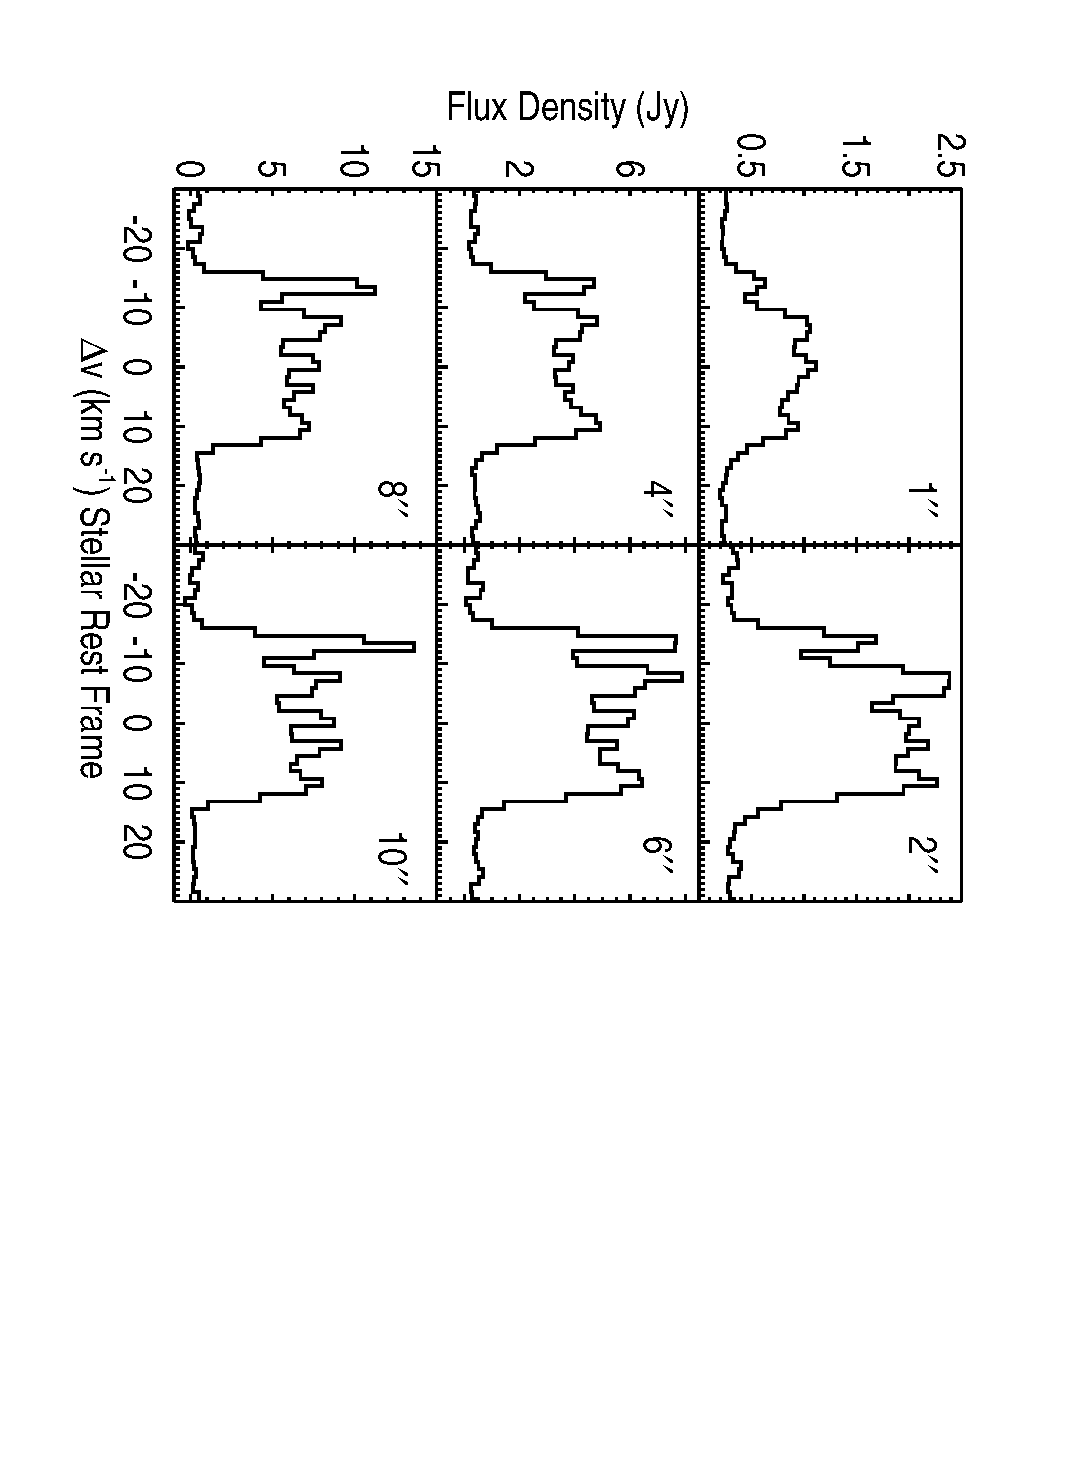
\includegraphics[trim=20pt 180pt 40pt 0pt, clip, angle=90, width=14.0cm, height=12.0cm]{/home/eamon/thesis/thesis_template/5/f2.eps}
\caption{Spectral profiles of the low spectral resolution multi-configuration image cube for circular extraction areas of radius 1$\arcsec$, 2$\arcsec$, 4$\arcsec$, 6$\arcsec$, 8$\arcsec$, and 10$\arcsec$. The signal-to-noise of the line profile reduces at larger extraction areas as more noise is included from the outer regions of the channel maps.}
\label{fig:5.5}
\end{figure}

The spectra in Figure \ref{fig:5.5} are taken from the low resolution multi-configuration image cube using circular extraction areas ranging in radius from 1$\arcsec$ to 10$\arcsec$ and demonstrates how the line profile changes over these different extraction areas. The most striking change in the line profile is the change in appearance of the extreme blue wing. At small extraction radii where we sample the most compact emission, the feature is weak in comparison to the rest of the line but becomes more dominant as we begin to sample more of the extended emission. This indicates that even the high absolute velocity components of the S2 flow have extended emission and this is why they are almost completely spatially filtered by CARMA's C configuration. The large reduction of flux at $-11\>{\rm km\>s}^{-1}$ suggests that there is more material moving towards the observer than at other lower absolute velocities indicating a non-isotropic (or non-spherical) S2 flow. This suggests a more sheet like (flatter) structure rather than a spherical cap.

\section{Individual Configuration Image Cubes}\label{sec:5.4}
2nd source
\section{Multi-configuration Image Cubes}\label{sec:5.5}
include \ion{K}{i} spectrum here
\section{Determination of S1 and S2 shell sizes}\label{sec:5.6} 
\section{Continuum Flux Densities}\label{sec:5.7}
\section{Higher CO rotational lines}\label{sec:5.8}
SOFIA, Hershel, SMA
\section{e-Merlin Results}\label{sec:5.8}
position, GMH model
\section{VLA Pi-Town vs e-Merlin}\label{sec:5.9}